%
% saddle-node.tex
%
% (c) 2018 Prof Dr Andreas Müller, Hochschule Rapperswil
%
\documentclass[tikz]{standalone}
\usepackage{times}
\usepackage{amsmath}
\usepackage{txfonts}
\usepackage[utf8]{inputenc}
\usepackage{graphics}
\usetikzlibrary{arrows,intersections}
\begin{document}

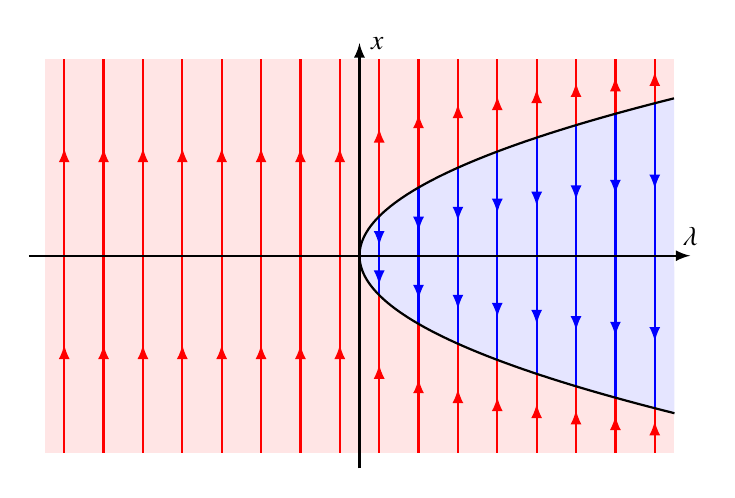
\begin{tikzpicture}[>=latex,thick]

\def\s{0.12}

\fill[color=red!10] (-4,-2.5)--(4,-2.5)--(4,2.5)--(-4,2.5)--cycle;

\fill[color=blue!10,domain=-2:2,samples=100]
	plot ({\x*\x},{\x});

\foreach \x in {-3.75,-3.25,...,-0.25}{
	\draw[->,color=red] (\x,-2.5)--(\x,-1.25+\s);
	\draw[->,color=red] (\x,-1.25)--(\x,1.25+\s);
	\draw[color=red] (\x,1.25)--(\x,2.5);
}
\foreach \x in {0.25,0.75,...,3.75}{
	\pgfmathparse{(sqrt(\x) + 2.5)/2}
	\edef\y{\pgfmathresult}
	\draw[->,color=red] (\x,{sqrt(\x)})--(\x,\y+\s);
	\draw[color=red] (\x,{\y})--(\x,2.5);
	\draw[->,color=red] (\x,-2.5)--(\x,{-\y+\s});
	\draw[color=red] (\x,{-\y})--(\x,{-sqrt(\x)});

	\draw[->,color=blue] (\x,{sqrt(\x)})--(\x,{sqrt(\x)/2-\s});
	\draw[->,color=blue] (\x,{sqrt(\x)/2})--(\x,{-sqrt(\x)/2-\s});
	\draw[color=blue] (\x,{-sqrt(\x)/2})--(\x,{-sqrt(\x)});
}

\draw[domain=-2:2,samples=100]
	plot ({\x*\x},{\x});

\draw[->] (-4.2,0)--(4.2,0) coordinate[label=$\lambda$];
\draw[->] (0,-2.7)--(0,2.7) coordinate[label={right:$x$}];

\end{tikzpicture}

\end{document}
